\documentclass{bschlangaul-aufgabe}
\bLadePakete{java,uml}
\begin{document}
\bAufgabenMetadaten{
  Titel = {Aufgabe 2},
  Thematik = {OOP/OOD - Reverse Engineering},
  Referenz = 66116-2015-F.T2-TA2-A2,
  RelativerPfad = Staatsexamen/66116/2015/03/Thema-2/Teilaufgabe-2/Aufgabe-2.tex,
  ZitatSchluessel = examen:66116:2015:03,
  BearbeitungsStand = mit Lösung,
  Korrektheit = unbekannt,
  Ueberprueft = {unbekannt},
  Stichwoerter = {Klassendiagramm},
  EinzelpruefungsNr = 66116,
  Jahr = 2015,
  Monat = 03,
  ThemaNr = 2,
  TeilaufgabeNr = 2,
  AufgabeNr = 2,
}

Leider ist das Klassendiagramm der folgenden Klassen verloren gegangen.
Führen Sie ein Reverse Engineering durch und erstellen Sie aus dem
Quellcode ein vollständiges UML-Klassendiagramm inklusive aller Klassen,
Schnittstellen, Attribute, Methoden, Konstruktoren, Sichtbarkeiten,
Assoziationen, Rollennamen, Multiplizitäten, Navigationspfeilen und
evtl. Stereotypen. Der Quellcode innerhalb von Methoden und
Konstruktoren soll nicht übertragen werden, wohl aber die
Methodensignaturen. Assoziationsnamen und deren Leserichtung lassen sich
aus dem Quellcode nur schwer erahnen und sollen deshalb ebenfalls
weggelassen werden.\index{Klassendiagramm}
\footcite{examen:66116:2015:03}

\def\j#1{\bJavaExamen{66116}{2015}{03}{reverse/#1}}

\j{Display}
\j{PixelPainter}
\j{HardwareMatrix}
\j{DisplayUnion}
\j{RGBDisplay}

\begin{bAntwort}
\begin{tikzpicture}

%%
%
%%

\umlclass[y=0,type=interface]{PixelPainter}
{}
{
  \~{}set(x : int, y : int, color : Color)\\
  \~{}getHeight() : int\\
  \~{}getWidth() : int
}

%%
%
%%

\umlclass[y=-4,type=abstract]{Display}
{
  %\#hardwareMatrix : HardwareMatrix\\
  \#lastPaintedX : int \\
  \#lastPaintedX : int \\
}
{
  +Display(hardwareMatrix : HardwareMatrix)\\
  +getWidth() : int\\
  +getHeight() : int\\
  +clear()\\
  \textit{\#getWidthFactor() : int}\\
  \textit{\#getHeightFactor() : int}\\
}

\umlimpl{Display}{PixelPainter}

%%
%
%%

\umlclass[y=-8,type=abstract]{RGBDisplay}
{}
{
  +RGBDisplay(matrix : HardwareMatrix)\\
  +set(x : int, y : int, color : Color)\\
  \#getWidthFactor() : int\\
  \#getHeightFactor() : int\\
}

\umlinherit{RGBDisplay}{Display}

%%
%
%%

\umlclass[y=-12]{DisplayUnion}
{
  \umlstatic{+MAX\_DISPLAY\_COUNT : int = 50 \{readOnly\}}\\
  -currentDisplayCount : int\\
  -displays : Display[1..50]\\
}
{
  +DisplayUnion(displays[1..50])\\
  +getDisplayCount() : int\\
  \#getWidthFactor() : int\\
  \#getHeightFactor() : int\\
  +set(x : int, y : int, color : Color)\\
}

\umlinherit{DisplayUnion}{RGBDisplay}

%%
%
%%

\umlclass[x=8,y=-4.1,type=interface]{HardwareMatrix}
{}
{
  \~{}set(x : int, y : int, v : int)\\
  \~{}getWidth() : int\\
  \~{}getHeight() : int\\
}

\umlassoc[arg2=\#hardwareMatrix,pos2=0.6]{Display}{HardwareMatrix}
\end{tikzpicture}
\end{bAntwort}

\end{document}
